\documentclass[../../../include/open-logic-section]{subfiles}

\begin{document}

\olfileid{sth}{ordinals}{idea}	
\olsection{క్రమసంఖ్య సాధారణ భావన}

సహజ సంఖ్యలను వాటి
సాధారణ క్రమంలో
పరిగణించండి:
\begin{center}
	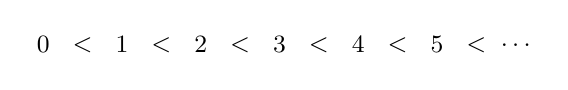
\begin{tikzpicture}
	\foreach \x/\xtext in {0, 1, 2, 3, 4, 5}
	{
		\node (\x a) at (\x, 1) {\small{$\x$}};
		\node (\x a) at (\x.5, 1) {\small{$<$}};
	}
	\node (ldots) at (6, 1) {\small{$\ldots$}};
	\end{tikzpicture}
\end{center}
సాంకేతిక భాషలో దీనిని
$\omega$-అనుక్రమం అంటాం.
నిజానికి సమితి స్థాయిక్రమపు
దశలను మనం మొదట
నిర్మించిన విధానంలోనూ
ఇదే సాధారణ క్రమం
కనిపిస్తుంది. అయితే
ఇప్పుడు $0$ను ఈ
అనుక్రమం చివరికి
మార్చి, మిగతా సంఖ్యలన్నింటి
తరువాత ఉంచుదాం:
\begin{center}
	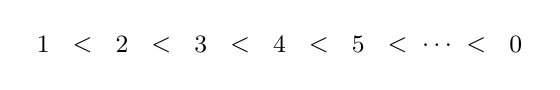
\begin{tikzpicture}
	\foreach \x/\xtext in {1, 2, 3, 4, 5}
	{
		\node (\x a) at (\x, 1) {\small{$\x$}};
		\node (\x a) at (\x.5, 1) {\small{$<$}};
	}
	\node (ldots) at (6, 1) {\small{$\ldots$}};
	\node (bea) at (6.5, 1) {\small{$<$}};
	\node (noa) at (7, 1) {\small{$0$}};
	\end{tikzpicture}
\end{center}
ఇక్కడ వస్తువులు అవే;
కానీ వాటి క్రమం
మౌలికంగా వేరుగా ఉంది:
మొదటి క్రమంలో చివరి
మూలకం లేదు; కొత్త
క్రమంలో ఉంది. నిజానికి
కొత్త క్రమంలో వస్తువుల
$\omega$-అనుక్రమం
($1, 2, 3, 4, 5, \ldots$)
తరువాత మరో వస్తువు
ఉంది. ఇది
$\omega+1$-అనుక్రమం.

ఇవే వస్తువులను వాడి
ఇంకా అనేక రకాల
క్రమాలను రూపొందించవచ్చు.
ఉదాహరణకు, సరి సంఖ్యలన్నింటిని
(వాటి సహజ క్రమంలో),
తరువాత బేసి సంఖ్యలన్నింటిని
(వాటి సహజ క్రమంలో)
పరిగణించండి:
\begin{center}
	\begin{tikzpicture}
	\node(a1) at (1,1) {\small{$0$}};
	\node(a2) at (1.5,1) {\small{$<$}};
	\node(a3) at (2,1) {\small{$2$}};
	\node(a4) at (2.5,1) {\small{$<$}};
	\node(a5) at (3,1) {\small{$4$}};
	\node(a6) at (3.5,1) {\small{$<$}};
	\node(dots) at (4,1) {\small{$\ldots$}};
	\node(aaoe) at (4.5,1) {\small{$<$}};
	\node(b1) at (5,1) {\small{$1$}};
	\node(b2) at (5.5,1) {\small{$<$}};
	\node(b3) at (6,1) {\small{$3$}};
	\node(b4) at (6.5,1) {\small{$<$}};
	\node(b5) at (7,1) {\small{$\ldots$}};
	\end{tikzpicture}
\end{center}
ఇది ఒక $\omega$-అనుక్రమం
తరువాత మరో $\omega$-అనుక్రమం;
అంటే $\omega+\omega$-అనుక్రమం.

ఇలా ఇంకా ముందుకు
వెళ్లవచ్చు. కానీ ఈ
\emph{క్రమాల} గురించిన
మాటను సాధారణంగా
అర్థం చేసుకునే ఒక
పద్ధతి మనకు కావాలి.

\end{document}
